\documentclass{article}
\usepackage[utf8]{inputenc}
\usepackage{tabularx}
\usepackage{graphicx}
\usepackage{amsmath,amssymb,hyperref,float}
\DeclareMathOperator*{\argmax}{arg\,max}
\newcommand{\R}{\mathbb{R}}
\newcommand{\N}{\mathbb{N}}
\DeclareMathOperator*{\argmin}{arg\,min}
\usepackage{geometry}
 \geometry{
 a4paper,
 total={170mm,257mm},
 left=20mm,
 top=20mm,
 }
 \graphicspath{ {./figs/} }


\title{IPCV}
\author{Dante Piotto}
\date{october 2022}

\begin{document}
\maketitle
\tableofcontents
\newpage
\section{Image formation and acquisition}

\subsection{pinhole camera}
simplest imaging device\\
geometrically, image is achieved by drawing straight lines from points in the scene through the pinhole to the image plane

\subsection{Perspective projection}
vars of intrest:
\begin{itemize}
	\item M(x,y,z): scene point
	\item m(u,v): corresponding image point
	\item I: image plane
	\item C: optical centre
	\item Line through C and orth to I: optical axis
	\item c: intersec between optical axis and image plane (piercing point/image center)
	\item f: focal length
	\item F: focal plane
\end{itemize}

equations that relate 3d obj coords (x,y,z) to image coords:
\begin{equation}
	\frac{u}{x} = \frac{v}{y}=- \frac{f}{z}
\end{equation}

to get rid of up/down and left/right inversions we can write
\begin{equation}
		u=  x \frac{f}{z}; \quad v=y \frac{f}{z}
\end{equation}

going from 3D to 2D implies a loss of information

\subsection{stereo vision}

Standard stereo geometry:\\
-Cameras arranged so that there is only horiz translation between the two CRF. Naming $b$ the distance between the two CRF the transformation between the CRF is
\begin{equation}
	p_L-p_R = \begin{bmatrix}
	b\\
	0\\
	0\\
	\end{bmatrix}
\end{equation}

with $p_L, p_R$ coords in left and right CRF\\
-same focal length for for both cameras (coplanar image planes)
\begin{gather*}
x_L-x_R=b\\
y_L=y_R=y\\
z_L=z_R=z\\
v_L=v_R=y \frac{f}{z} (*)\\
u_L=x_L \frac{f}{z}\\
u_R=x_R \frac{f}{z}\\
\Rightarrow u_L-u_R=b \frac{f}{z}\\
u_L-u_R=d (disparity)\\
\Rightarrow d=b \frac{f}{z}\\
\Rightarrow z = b \frac{fe}{d}
\end{gather*}

eq. for y(*) helps solve correspondence as corresponding points have the same y coord in both images $\Rightarrow$ better efficiency and lower risk of mistakes due to smaller search set
\subsection{Epipolar geometry}
The search space of the stereo correspondence problem is always 1D because all possible 3D points that can be correspondent to a pixel lie along a line (optical ray)\\
epipolar line: projection of an optical ray of one camera onto the image of the other (useful if not in standard stereo geometry)\\
Standard stereo geometry is more computationally efficient\\
Dense depth map: image in which depth is known for every pixel\\
images from epipolar cameras can be rectified for computational efficiency

\subsection{properties of perspective projection}
\begin{itemize}
	\item the transformation is non-linear
	\item perspective projection maps 3D lines into image lines (straight)
	\item ratios of length are not preserved unless the scene is planar and parallel to the image plane
	\item parallelism between 3D lines is not preserved: they converge in a vanishing point unless the lines are in a plane parallel to the image plane \begin{itemize}
		\item the vanishing point of a 3D line is the image of the point at infinity of the line
		\item that is the intersection of between the parallel to the line passing through the optical center and the image plane
	\end{itemize}
	
\end{itemize}

A scene point is in focus when all its light rays converge into a single point: always true for pinhole camera. Drawback: long exposure time is needed due to infinitesimal pinhole and scene has to be static.\\
Solution: lenses that gather light and focus it in a single point
\subsection{thin lens model}
\begin{equation}
	\frac{1}{u}+\frac{1}{v}=\frac{1}{f}
\end{equation}
\begin{itemize}
	\item rays parallel to the optical axis are deflected to pass through F
	\item rays through C are undeflected
\end{itemize}
If the image is in focus, the image formation process obeys the perspective projection model, with the center of the lens being the optical center and the distance $v$ acting as the effective focal length of the projection\\
given an image distance, 1 scene plane is in focus\\
scene points outside the focusing plane are mapped into circles of confusion/blur circles\\
this problem is alleviated in some ways: 
\begin{itemize}
	\item method of acquisition (if blur circle is small enough it falls into one pixel)
	\item lens size (smaller lenses $\rightarrow$ smaller blur circles)
	\item diaphragm (affects effective lens size used)
\end{itemize}
F number = ratio of focal length to effective aperture ($f/d$)\\
focusing mechanism: lens is moved wrt the image plane (sensor)

\subsection{Image digitization}
Sensor converts irradiance into an electric quantity (e.g. voltage), which is sampled (2D array of pixels) and quantized (typically 8 bit in grayscale $\rightarrow$ 256 levels)\\
In practice image is sampled when sensed due to arrays being arranged in an array\\
In digital cameras sensor array=pixels\\
In analog cameras image from sensor array s conveerted to analog signal and then reconverted to digital but pixels $\neq$ camera sensor array\\
sensors are typically CCD or CMOS\\
CCD/CMOS is not sensitive to light wavelength $\rightarrow$ colour filtering arrays (CFA)

\subsection{Camera parameters}
\begin{itemize}
	\item Signal to Noise Ratio (SNR). Main noise sources: \begin{itemize}
		\item Photon Shot Noise: number of photons collected during exposure time is random (Poisson statistics)
		\item Electronic Circuitry Noise
		\item Quantization Noise: related to ADC conversion (in digital cameras)
		\item Dark Current Noise: a random amount of charge is generated in photocapacitors in the dark due to thermal excitement. A lower bound $E_{min}$ is set on the detected irradiation
	\end{itemize}
	\item Dynamic Range (DR): $E_{max}$= irradiation that would fill up the capacity of a photodetector \begin{itemize}
		\item $DR=\frac{E_{max}}{E_{min}}$
		\end{itemize}
	\item Sensitivity: amount of signal the sensor can deliver per unit of input optical energy
	\item Uniformity: responses to light and dark noise vary from pixel to pixel
\end{itemize}
both SNR and DR are usually specified in decibels or bits\\
CCD typically provides higher SNR, DR, and better uniformity than CMOS\\
with CMOS electronics can be integrated on the same chip $\rightarrow$ compactness, power efficiency, lower cost.\\
With CMOS an arbitrary window can be read out without having to receive the full image\\
To create colour an array of CFAs is placed in front of the photodetectors so as to render each pixel sensitive to a specific range of wavelengths

\subsection{Perspective projection}
By appending a 1 to the Euclidean coordinates of the object we obtain the coordinates in the projective space $\mathbb{P}^3$. We assume
\begin{equation}
	(x \quad y \quad z \quad\ 1)=(kx \quad ky \quad kz \quad\ k) \forall k \neq 0
\end{equation}
these are called homogeneous coordinates (aka projective coordinates) representation of the 3D point having Euclidian coordinates (x,y,z)

\subsubsection{Point at infinity of a 3D line}
Considering the parametric equation of a 3D line:
\begin{equation}
	M = M_0 + \lambda D = \begin{bmatrix}
	x_0\\
	y_0\\
	z_0
	\end{bmatrix} + \lambda \begin{bmatrix}
	a\\
	b\\
	c
	\end{bmatrix} = \begin{bmatrix}
	x_0 + \lambda a \\
	y_0 + \lambda b \\
	z_0 + \lambda c 
	\end{bmatrix}
\end{equation}
in projective coordinates
\begin{equation}
	\tilde{M} = \begin{bmatrix}
	M\\
	1
	\end{bmatrix} = \begin{bmatrix}
	x_0 + \lambda a \\
	y_0 + \lambda b \\
	z_0 + \lambda c \\
	1
	\end{bmatrix} = \begin{bmatrix}
	\frac{x_0}{\lambda} + a\\
	\frac{y_0}{\lambda} + b\\
	\frac{z_0}{\lambda} + c\\
	\frac{1}{\lambda}
	\end{bmatrix}
\end{equation}
by taking the limit with $\lambda \rightarrow \infty$ we obtain the projective coordinates of the point at infinity of the given line:
\begin{equation}
	\tilde{M}_{\infty}= \lim_{\lambda \to \infty} \tilde{M} = \begin{bmatrix}
	a\\
	b\\
	c\\
	0
	\end{bmatrix}
\end{equation}

\begin{itemize}
	\item to map points at infinity from the projective space to the Euclidean space we would divide by the fourth coordinate (0)
	\item point (0,0,0,0) is undefined
        \item it can be shown that all points at infinity in $\mathbb{P}^3$ lie on a plane called plane at infinity
\end{itemize}

\subsubsection{Perspective projection in projective coordinates}
\begin{gather}
	u=\frac{f}{z} x \qquad v=\frac{f}{z} y \\
	M= [x,y,z]^T \qquad m=[u,v]^T \\
	\tilde{M} = [x,y,z,1]^T \qquad \tilde{m} = [u,v,1]^T\\
	\begin{bmatrix}
	u\\
	v\\
	1
	\end{bmatrix} = \begin{bmatrix}
	f \frac{x}{z}\\
	f \frac{y}{z}\\
	1
	\end{bmatrix} = \begin{bmatrix}
	fx\\
	fy\\
	z
	\end{bmatrix} = \begin{bmatrix}
	f & 0 & 0 & 0\\
	0 & f & 0 & 0\\
	0 & 0 & 1 & 0\\
	\end{bmatrix} \begin{bmatrix}
	x\\
	y\\
	z\\
	1
	\end{bmatrix}
\end{gather}
or in matrix notation
\begin{equation}
	k \tilde{m} = \tilde{P} \tilde{M}
\end{equation}
often expressed as 
\begin{equation}
	\tilde{m} \approx \tilde{P} \tilde{M}
\end{equation}
where $\approx$ means "equal up to an arbitrary scale factor"\\
if we assume distances to be measured in focal lengths ($f=1$), the PPM becomes
\begin{equation}
    \tilde{P}= \begin{bmatrix}
        1 & 0 & 0 & 0 \\
        0 & 1 & 0 & 0 \\
        0 & 0 & 1 & 0 
    \end{bmatrix}=[I_3|0]
\end{equation}
called the canonical PPM
\subsection{Building a useful camera model}
For a useful camera model we need to take into account:
\begin{itemize}
    \item Image digitization
    \item rototranslation between the CRF (camera reference frame) and the WRF (world reference frame)
\end{itemize}
\subsubsection{Image digitization}
Digitization can be accounted for by including into the projection equations the scaling factors along the two axes due to the quantization associated with the horizontal and vertical pixel size ($\Delta u$ and $\Delta v$). We also need to model the translation of the piercing point wrt the origin of the image coordinate system
\begin{gather*}
    u=\frac{f}{z}x \quad \rightarrow u = \frac{1}{\Delta u} \frac{f}{z}x=k_u\frac{f}{z}x+u_0 \\
    v=\frac{f}{z}y \quad \rightarrow v = \frac{1}{\Delta v} \frac{f}{z}x=k_v\frac{f}{z}x+u_0 \\
\end{gather*}
The PPM can therefore be rewritten as
\begin{equation}
    \tilde{P}=\begin{bmatrix}
        fk_u & 0 & u_0 & 0 \\
        0 & fk_v & v_0 & 0 \\
        0 & 0 & 1 & 0
    \end{bmatrix}=\begin{bmatrix}
        fk_u & 0 & u_0 \\
        0 & fk_v & v_0 \\
        0 & 0 & 1
    \end{bmatrix} \begin{bmatrix}
        1 & 0 & 0 & 0 \\
        0 & 1 & 0 & 0 \\
        0 & 0 & 1 & 0 
    \end{bmatrix} = A[I|0]
\end{equation}

Matrix A, which models the characteristics of the camera, is called \emph{Intrinsic Parameter Matrix}\\
$fk_u=\alpha_u$ and $fk_v=\alpha_v$ are called horizontal and vertical scale factors
\subsubsection{Rigid motion between CRF and WRF}
The WRF can be related to the CRF by:
\begin{itemize}
    \item a rotation around the optical centre (3x3 rotation matrix $R$)
    \item a translation (3x1 translation vector $T$)
\end{itemize}
Therefore, the relation between coords of a point in the 2 RF is:
\begin{equation}
    W=\begin{bmatrix}
        X\\
        Y\\
        Z
    \end{bmatrix},M=\begin{bmatrix}
        x\\
        y\\
        z
    \end{bmatrix} \Rightarrow M=RW+T
\end{equation}
in homogenous coordinates:
\begin{equation}
    \tilde{W}=\begin{bmatrix}
        X\\
        Y\\
        Z\\
        1
    \end{bmatrix}, \tilde{M}= \begin{bmatrix}
        x\\
        y\\
        z\\
        1
    \end{bmatrix} \Rightarrow \tilde{M} = \begin{bmatrix}
        R & T\\
        0 & 1\\
    \end{bmatrix} \tilde{W}=G\tilde{W}
\end{equation}

A 3D point is therefore mapped into the CRF as
\begin{equation}
    k\tilde{m}=A[I|0]\tilde{M}
\end{equation}
by considering the rigid body motion between WRF and CRF:
\begin{gather}
    \tilde{M} = G \tilde{W} \rightarrow k\tilde{m}=A[I|0]G\tilde{W}\\
    k\tilde{m}=A[I|0]\begin{bmatrix}
        R & T \\
        0 & 1 \\
    \end{bmatrix} \tilde{W}
\end{gather}
Accordingly, the general form of the PPM can be expressed as:
\begin{equation}
    \tilde{P} = A[I|0]G \quad \text{or also} \quad \tilde{P}=A[R|T]
\end{equation}
Matrix G, which encodes the position and orientation of the camera wrt the WRF, is called Extrinsic Parameter Matrix\\
To be noted: the actual DoFs of G are 6, 3 due to rotation and 3 due to translation

\subsection{Homographies}
\subsubsection{P as a Homography} \label{sec:homo}
If the camera is imaging a planar scene we can assume the z axis of the WRF to be perpendicular to the plane so that all points have z coordinate 0. The PPM simplifies as follows:
\begin{equation}
    k\tilde{m}=\tilde{P}\tilde{W}=\begin{bmatrix}
        p_{11} & p_{12} & p_{13} & p_{14} \\
        p_{21} & p_{22} & p_{23} & p_{24} \\
        p_{31} & p_{32} & p_{33} & p_{34} 
    \end{bmatrix} \begin{bmatrix}
        x\\
        y\\
        0\\
        1
    \end{bmatrix}=\begin{bmatrix}
        p_{11} & p_{12} & p_{14} \\
        p_{21} & p_{22} & p_{24} \\
        p_{31} & p_{32} & p_{34}
    \end{bmatrix} \begin{bmatrix}
        x\\
        y\\
        1
    \end{bmatrix}=H\tilde{M}
\end{equation}
where H is denoted as a \emph{homography}, i.e. a linear transformation between projective planes.\\
Akin to P, H is known up to an \emph{arbitrary scale factor} and thus independent elements in H(3x3) are just 8.\\
H is always invertible\\
Further examples of cases where homographies are applicable:
\begin{itemize}
    \item two images of a planar scene
    \item two images taken by a camera rotating about the optical centre
    \item two images taken by different cameras (i.e. different A) in a fixed pose (i.e. same CRF)
    \item two images taken by different cameras rotated about the optical centre
\end{itemize}

\subsection{Lens distortion}
Lens distortion is modelled through additional parameters that don't alter the form of the PPM
\begin{itemize}
    \item Radial distortion: points at the same distance from the centre of distortion (radius) are affected in the same way by the distortion, and distortion grows with the radius. Can be split into: \begin{itemize}
        \item barrel distortion
        \item pincushion distortion
    \end{itemize}
    \item tangential distortion: due to misalignment of optical components and/or defects
\end{itemize}
Distortion is modelled through a non-linear mapping between ideal image coordinates and observed (distorted) image coordinates, which is a mapping between \emph{CONTINUOUS} coordinates
\begin{equation}
    \begin{bmatrix}
        x'\\
        y'
    \end{bmatrix}=L(r)\begin{bmatrix}
        \tilde{x}\\
        \tilde{y}
    \end{bmatrix}+\begin{bmatrix}
        d\tilde{x}\\
        d\tilde{y}
    \end{bmatrix}
\end{equation}
$(x', y')$ are the distorted coordinates and $(\tilde{x},\tilde{y})$ are the undistorted coordinates, r is the distance from the distortion centre $(x_c, y_c)$ $r=\sqrt{(x-x_c)^2+(y-y_c)^2}$\\
The first term regards radial distortion, while the second deals with tangential distortion\\
$L(r)$ is usually approximated by its Taylor series around the centre of distortion $(r=0)$
\begin{equation}
    L(r)=1+k_1r^2+k_2r^4+k_3r^6+\dots
\end{equation}
$L(0)=1$, therefore there is no distortion at the centre of distortion. The odd terms are not present beacause $L(r)$ is undefined for $r<0$, so it can be considered to be an even function.

Tangential distortion is approximated as follows:
\[
    \begin{bmatrix}
        d\tilde{x}\\ d\tilde{y} 
    \end{bmatrix} = \begin{bmatrix}
        2p_1\tilde{x}\tilde{y}+p_2(r^2+2\tilde{x}^2)\\
        p_1(r^2+2\tilde{y}^2)+2p_2\tilde{x}\tilde{y}
    \end{bmatrix}
\]
\section{Camera calibration}
for the sake of camera calibration, patterned surfaces such as checkboards are used to find corresponding points.
\subsection{Zhang's Method}
\begin{enumerate}
    \item Acquire n images of a planar pattern with m internal corners
    \item Compute a homography $H_i$ for each image

        Due to the calibration pattern being planar and the choice of the WRF associated with the calibration images, for each of them we consider only 3D control points with $z=0$. Therefore, the mapping between 3D coordinates of the control points and their projections in the calibration images is a homography (see section \ref{sec:homo}):
        \[
            k\tilde{m} = \tilde{P}\tilde{w} =  H\tilde{w}'
        \]
        Given a pattern with $m$ corners, we can write $m$ systems of 3 linear equations as above, wherein both 3D (with $z=0$) as well as 2D coordinates are known due to corners having been detected in the calibration image and the uknowns being therefore only the elements in $H$
    \item Refine each $H_i$ by minimizing the reprojetion error

        Given the previous initial estimation, $H_i$ is later refined by the least-squares solution of the non-linear minimization problem 
        \[
            H = \argmin_{H\in\R^9} \displaystyle\sum_{j=1}^{m} \|\tilde{m}_j - H\tilde{w}_j'\|^2
        \]
        which can be obtained by using the Levenberg-Marquardt algorithm. The previous step is necessary to initialize the problem close to a solution
    \item given all the $H_i$ get an initial guess for the intrinsics A

        As $H$ is known up to a scale factor, we can establish the following relation beteen $H$ and the PPM:
        \[
            H = \begin{bmatrix}
                h_1 & h_2 & h_3
            \end{bmatrix} = \begin{bmatrix}
                p_1 & p_2 & p_4
            \end{bmatrix} = \lambda A \begin{bmatrix}
                r_1 & r_2 & T
            \end{bmatrix}
        \]
        $R$ is an orthonormal matrix. This constrains the intrinsic parameters to obey the following relations:
        \begin{align*}
            &&r_1^T r_2 = 0 & \implies h_1^T A^{-T}A^{-1} h_2 = 0\\
            &&r_1^T r_1 = r_2^T r_2 & \implies h_1^T A^{-T}A^{-1} h_1 = h_2^T A^{-T}A^{-1} h_2
        \end{align*}
        where the uknowns are the entries of $B=A^{-T}A^{-1}$. As $A$ is upper triangular, $B$ turns out to be symmetric, so there are only 6 uknowns. By stacking the above two equations provided by each calibration image, we obtain a $2n\times 6$ linear system, which can be solved in case at least 3 images are available.
    \item Given A and $H_i$ get an initial guess for $R_i$ and $T_i$ (extrinsics)

        \begin{align*}
            H = \begin{bmatrix}
                h_1 & h_2 & h_3
            \end{bmatrix} = \lambda A \begin{bmatrix}
                r_1 & r_2 & T 
            \end{bmatrix} \\
           h_1 = \lambda A r_1 \implies r_1 = \displaystyle\frac{1}{\lambda} A^{-1} h_1
        \end{align*}
      As $r_1$ is a unit vecotr:
        \[
            \lambda = \|A^{-1} h_1\|, \quad r_2 = \displaystyle\frac{1}{\lambda} A^{-1} h_2
        \]
        $r_3$ can be derived from $r_1$ and $r_2$ by exploiting orthonormality:
        \[
            r_3 = r_1 \times r_2
        \]
        Finally we can get $T$:
        \[
            T = \displaystyle\frac{1}{\lambda} A^{-1} h_3
        \]
    \item compute an initial guess for lens distortion k

        Given the already know intrinsic parameter matrix $A$, and the lens distortion model:
        \[
            \begin{bmatrix}
                x'\\
                y'
            \end{bmatrix} = L(r) \begin{bmatrix}
                \tilde{x}\\
                \tilde{y}
            \end{bmatrix} =(1 + k_1 r^2 + k_2 r^4) \begin{bmatrix}
                \tilde x\\
                \tilde y
            \end{bmatrix}
        \]
        we need to first establish the relationship between the distorted ($u',v'$) and ideal ($\tilde u,\tilde v$) pixel coordinates:
        \[
            \begin{bmatrix}
                u' \\ v' \\ 1
            \end{bmatrix} = A \begin{bmatrix}
                x' \\ y' \\ 1
            \end{bmatrix} = \begin{bmatrix}
                \alpha_u & 0 & u_0 \\
                0 & \alpha_v & v_0 \\
                0 & 0 & 1
            \end{bmatrix} b \begin{bmatrix}
                x' \\ y' \\ 1
            \end{bmatrix}
        \rightarrow \begin{cases}
            \displaystyle\frac{u' - u_0}{\alpha_u} = (1 + k_1 r^2 + k_2 r^4) \left(\displaystyle\frac{\tilde u - u_0}{\alpha_u} \right)\\
            \displaystyle\frac{v' - v_0}{\alpha_v} = (1 + k_1 r^2 + k_2 r^4) \left(\displaystyle\frac{\tilde v - v_0}{\alpha_v} \right)\\
        \end{cases}
    \]
    It is therefore possible to set up a linear system where the unknowns are the distortion coefficients: 
    \[
        \begin{bmatrix}
            (\tilde u - u_0) r^2 & (\tilde u - u_0) r^4 \\
            (\tilde v - v_0) r^2 & (\tilde v - v_0) r^4
        \end{bmatrix} \begin{bmatrix}
            k_1 \\ k_2 
        \end{bmatrix} = \begin{bmatrix}
            u' - \tilde u \\
            v' - \tilde v
        \end{bmatrix} \qquad \qquad r^2 = \left(\displaystyle\frac{\tilde u - u_0}{\alpha_u}\right)^2 + \left(\displaystyle\frac{\tilde v - v_0}{\alpha_v}\right)^2
    \]
    With $m$ corner features in $n$ images, we get a linear system with $2mn$ equations in 2 unknowns, which admits a least-squares solution:
    \[
        Dk =d \implies k = D^\dagger d = (D^TD)^{-1}D^Td
    \]
    \item refine A, $R_i$, $T_i$, k by minimizing the reprojection error
        This is again done using the Levenberg-Marquardt algorithm to minimize the reprojection error
        \[
            \displaystyle\sum_{i=1}^{n} \displaystyle\sum_{j=1}^{m} \|m_{ij} - \hat{m}(A,k,R_i,T_i,w_j)|^2
        \]
\end{enumerate}

Given a planar chessboard pattern, known are:
\begin{itemize}
    \item the number of internal corners of the pattern, different along the two orthogonal directions for the sake of disambiguation
    \item The size of the squares which form the pattern
\end{itemize}
Internal corners can be detected easily by standard algorithms (e.g. Harris corner detector). In each image, the 3D WRF is taken at the top-left corner of the pattern, with plane $z=0$ given by the pattern itself and the $x,y$ axes alingned to the two orthogonal directions, in particular so as to always keep the same association between axes and directions. Thus, as for 3D points:
\begin{itemize}
    \item The third coordinate is always 0 
    \item $x$ and $y$ are determined by the known size of the squares forming the chessboard 
\end{itemize}
To get camera parameters, two main steps are carried out: 
\begin{itemize}
    \item Initial guess by a linear optimizer (minimization of an algebraic error) 
    \item Refinement by a non-linear optimizer (minimization of a geometric error)
\end{itemize}
% [TODO] make image
Each image requires its own estimate of the extrinsic parameters, as they differ from image to image. A global WRF can be taken to coincide with that associated with one of the calibration images, e.g. the first.

\subsection{Calibration of a stereo camera [INCOMPLETE]}
The two cameras can be separately calibrated using Zhang's algorithm.\\
Rototranslation between the two cameras needs to be calibrated

\section{Image filtering}
Image filter: image processing algorithm that computes the new intensity (colour) of a pixel p based on intensities (colours) of pixels in its neighbourhood
\subsection{Linear Translation-Equivariant filters}
Given an input 2D signal $i(x,y)$, a 2D operator $T\{\cdot\}:o(x,y)=T\{i(x,y)\}$ is said to be linear iff:
$$T\{ai_1(x,y)+bi_2(x,y)\}=ao_1(x,y)+bo_2(x,y)$$ with $o_1(\cdot)=T\{i_1(\cdot)\}, o_2(\cdot)=T\{i_2(\cdot)\}$ and a,b constants.\\
$T\{\cdot\}$ is said to be translation-equivalent iff:
$$T\{i(x-x_0,y-y_0)\}=o(x-x_0,y-y_0)$$
If the operator is LTE, the output signal is given by the convolution between the impulse response (point spread function), $h(x,y)=T\{\delta(x,y)\}$ of the operator and the input signal.
$$o(x,y)=T\{i(x,y)\}=\int_{-\infty}^{+\infty} \int_{-\infty}^{+\infty} i(\alpha,\beta)h(x-\alpha,y-\beta)d\alpha d\beta$$\\
LTE filters can be expressed through convolutions

\subsection{Convolution}
\subsubsection{Properties of convolution}
\begin{itemize}
    \item Associative property
    \item Commutative property
    \item Distributivity wrt sum
    \item Commutation with differentiation $(f*g)'=f'*g=f*g'$
\end{itemize}
\subsubsection{Correlation}
The correlation of signal $i(x,y)$ wrt signal $h(x,y)$ is:
$$i(x,y)\circ h(x,y) = \int_{-\infty}^{+\infty} \int_{-\infty}^{+\infty} i(\alpha,\beta)h(x+\alpha,y+\beta)d\alpha d\beta$$
Correlation is not commutative.\\
If h is an even function ($h(x,y)=h(-x,-y)$):
\begin{gather*}
    i(x,y)*h(x,y)=h(x,y)*i(x,y)=\int_{-\infty}^{+\infty} \int_{-\infty}^{+\infty} i(\alpha,\beta)h(x-\alpha,y-\beta)d\alpha d\beta\\
    = \int_{-\infty}^{+\infty} \int_{-\infty}^{+\infty} i(\alpha,\beta)h(\alpha-x,\beta-y)d\alpha d\beta\\
    = h(-x,-y)\circ i(x,y) = h(x,y) \circ i(x,y)
\end{gather*}
hence if h is even, the convolution between i and h is the same as the correlation of h wrt i.
\subsubsection{Discrete convolution}
For discrete signals, convolution is defined as follows:
\begin{equation}
    O(i,j)=T\{I(i,j)\}=\sum_{m=-\infty}^{+\infty} \sum_{n=-\infty}^{+\infty} I(m,n)H(i-m,j-n)
\end{equation}
where $I(i,j)$ and $O(i,j)$ are the discrete 2D input and output signals and $H(i,j)=T\{\delta(i,j)\}$ is the kernel of the LTE operator, i.e. the response to the 2D discrete unit impulse (Kronecker delta function) $\delta(i,j)$. Properties of convolution hold in the discrete case.
\subsubsection{Practical implementation of discrete convolution}
Due to the image being much larger than the kernel, commutativity is exploited in order to obtain a more efficient implementation of convolution:
\begin{equation}
    O(i,j)=T\{I(i,j)\}=\sum_{m=-k}^{k} \sum_{n=k}^{k} K(m,n)I(i-m,j-n)
\end{equation}
This equates to sliding the kernel across the whole input image and computing the convolution at each pixel. Pixels close to the border will lack some pixels for the computation of the convolution that would be outside the image. There are two main solutions:
\begin{itemize}
    \item CROP: common in image processing, bad with chains of convolution
    \item PAD: zero padding, replicate, reflect, reflect\_101
\end{itemize}
Computational cost: $(2k+1)^2$ MADs, $2(2k+1)^2$ operations per pixel.

\section{Denoising}
\subsection{Taking a mean across time}
The output at point p is:
\begin{equation}
    O(p)=\frac{1}{N} \sum_{k=1}^N I_k(p) = \frac{1}{N} \sum_{k=1}^N (\tilde{I}(p)+n_k(p)) = \frac{1}{N} \sum_{k=1}^N \tilde{I}(p) + \frac{1}{N} \sum_{k=1}^N n_k(p) \cong \tilde{I}(p)
\end{equation}
where $\tilde{I}(p)$ is the ideal undisturbed signal and $n_k(p)$ is the noise by which the signal is affected. Tipycally though, only a single image is available, therefore this approach is not feasible. 
\subsection{Mean Filter}
If we are given a single image, we may compute a mean across neighbouring pixels, i.e. a spatial mean. Mean filtering is the simplest and fastest way to denoise an image. It consists in replacing each pixel intensity with the average intensity over a chosen (square) neighbourhood. The Mean Filter is an LTE operator as it can be expressed as a convolution with a kernel, e.g. for a  3x3 mean filter:
\[
    \begin{bmatrix}
        1/9 & 1/9 & 1/9 \\
        1/9 & 1/9 & 1/9 \\
        1/9 & 1/9 & 1/9
        \end{bmatrix} = \frac{1}{9} \begin{bmatrix}
        1 & 1 & 1 \\
        1 & 1 & 1 \\
        1 & 1 & 1 
    \end{bmatrix}
\]
According to signal theory, the Mean Filter carries out a \emph{low pass filtering} operation, which is referred to in image processing as \emph{image smoothing}. Smoothing is ofthen aimed at denoising, though sometimes its purpose is to cancel out small-size unwanted details that might hinder image analysis. Mean filtering is inherently fast as multiplications are not needed. Moreover, it can be implemented very efficiently by incremental calculation schemes (Box-filtering)
\subsubsection{Box-Filtering}
Given boxes of size $2k+1$
\[
    \mu (i,j) = \frac{\sum_{m=-k}^{n=k}\sum_{n=-k}^{n=k} I(i+m,j+n)}{(2k+1)^2}=  \frac{s(i,j)}{2k+1)^2}
\]
Where
\[
    s(i,j+1)=s(i,j)+V^+(i,j+1)-V^-(i,j+1)
\]
and 
\begin{gather*}
    V^+(i,j+1)=V^+(i-1,j+1)+a-b\\
    V^-(i,j+1)=V^-(i-1,j+1)+c-d\\
    V^+(i,j+1)-V^-(i,j+1)=\Delta(i,j+1)
\end{gather*}
Resulting in
\[
    s(i,j+1)=s(i,j)+\Delta(i-1,j+1)+a-b-c+d
\]

Insert image from slides

We therefore have only 5 sums per pixel, independently of kernel size.

\subsection{Gaussian Filter}
LTE operator whose impulse response is a 2D Gaussian function (with zero mean and constant diagonal covariance matrix). The paramenter $\sigma$ sets the amount of smoothing. As $\sigma$ gets larger, the amount of smoothing grows.

The discrete Gaussian kernel can be obtained by sampling the corresponding continuous function, which is however of infinite extent. A finite size must be properly chosen. As the interval $[-3\sigma, +3\sigma]$ captures 99\% of the area of the Gaussian function, a typical rule of thumb dictates taking a $(2k+1)\times(2k+1)$ kernel with $k=3\lceil \sigma \rceil$.
It can be noted that, as the size of the kernel grows:
\begin{itemize}
    \item the more accurate the discrete approximation of the ideal filter turns out
    \item the more the computational cost grows
    \item the Gaussian gets smaller and smaller as we move away from the origin
\end{itemize}
\subsubsection{deploying separability}
To further speed up computation, one may observe that the 2D Gaussian is the product of two 1D Gaussians, therefore the original 2D convolution may be split into the chain of two 1D convolutions along $x$ and along $y$
\begin{gather}
    I(x,y) \ast G(x,y) = \int_{-\infty}^{+\infty}\int_{-\infty}^{+\infty}I(\alpha,\beta)G(x-\alpha,y-\beta)d\alpha d\beta\\
    G(x,y)=G(x)G(y)\\
    I(x,y)\ast G(x,y) = \int_{-\infty}^{+\infty}\int_{-\infty}^{+\infty} I(\alpha,\beta)G(x-\alpha)G(y-\beta)d\alpha d\beta\\
    I(x,y)\ast G(x,y) = \int_{-\infty}^{+\infty}G(y-\beta)\left(\int_{-\infty}^{+\infty} I(\alpha,\beta)G(x-\alpha)d\alpha \right) d\beta\\
    I(x,y)\ast G(x,y) = (I(x,y)\ast G(x))\ast G(y) = (I(x,y) \ast G(y)) \ast G(x)
\end{gather}
The speed-up brought in by the separability property can be expressed as:
\begin{gather}
    \text{2D Filter: } N_{OPS} = 2\times(2k+1)^2\\
    \text{1D Filter: } N_{OPS} = 2\times2\times(2k+1)\\
    S=\frac{2\times(2k+1)^2}{ 2\times2\times(2k+1) } = k+ \frac{1}{2}
\end{gather}
\subsection{Median Filter}
A non-linear filter whereby each pixel intensity is replaced by the median over a given neighbourhood. Median filtering counteracts impulse noise effectively, as outliers tend to fall at either the top or bottom of the sorted intensities. Median filtering also tends to keep sharper edges than linear filters such as the mean or gaussian, it cannot however correct Gaussian-like noise. A standard preprocessing pipeline includes first a median filter followed by a gaussian filter.
\subsection{Bilateral Filter}
An advanced non-linear filter to accomplish the denoising of a Gaussian-like noise without blurring the image (aka \emph{edge preserving smoothing}). The kernel is computed based on the distance from the considered pixel and the difference in intensity.
\[
    O(p)=\sum_{q\in S} H(p,q)I_q
\]
where $H(p,q)$ is a weighing function of p(central pixel) and q(neighbour pixel)
\[
    H(p,q) = \frac{1}{W(p)}G_{\sigma_s}(d_s(p,q))G_{\sigma_r}(d_r(I_p,I_q))
\]
where $G_{\sigma_s}$ is the spatial Gaussian, $G_{\sigma_r}$ is the intensity Gaussian, $d_s$ is the spatial distance, $d_r$ is the range (intensity distance), and $W(p)$ is the Normalization Factor
\begin{gather*}
    d_s(p,q) = \|p-q\|_2 = \sqrt{(u_p-u_q)^2+(v_p-v_q)^2}\\
    d_r(I_p,I_q) = |I_p-I_q|\\
    W(p)= \sum_{q\in S} G_{\sigma_s}(d_s(p,q))G_{\sigma_r}(d_r(I_p,I_q))
\end{gather*}
\subsection{Non-local Means Filter}
A non-linear edge preserving smoothing filter. It considers similarities among neighbourhoods spread over the image
\[
    O(p) = \sum_{q\in I}w(p,q)I(q)
\]
where
\begin{gather*}
    w(p,q)=\frac{1}{Z(p)}e^{-\frac{\|N_p-N_q\|^2_2}{h^2}}\\
    Z(p) = \sum_{q\in I} e^{-\frac{\|N_p-N_q\|^2_2}{h^2}}
\end{gather*}
In practice, to reduce the computational burden, only a region of the image is considered rather than the whole image.






\section{Image segmentation and blob analysis} 
Segmentation consists of dividing an image in foreground and background regions, an labelling different objects in the foreground.
Binarization is the division of the image into foreground and background based on pixel intensity, while labelling is finding connected components of a binary image. 
\subsection{Binarization}
Binarization is obtained through the gray-level histogram, which is a function associating to each gray level the number of pixels that have that level. It can only be done for inherently inherently binary images. 

Normalizing the histogram provides the relative frequencies of gray levels in the image. The normalized histogram can be thought of as the probability mass function (pmf) of the discrete random variable given by the gray level of a randomly picked pixel in the image. Binarization can be done by thresholding the gray level of pixels based on the information given by the gray-level histogram. 

\subsubsection{Automatic threshold selection}
\paragraph{Mean of gray level}
only works if the pixels are equally distributed between foreground and background
\paragraph{Peaks method}
\[
    T = \argmin\left\{h(i) | i \in [i_1, i_2]\right\}
\]
requires finding the two main peaks, which often implies smoothing the histogram before looking for peaks to aveoid the searchg being trapped into spurious local maxima. Two find the two main peaks, 3-level or 5-level neighbourhoods are used.
\paragraph{Otsu's Algorithm}
Let us define:
\begin{itemize}
    \item $i=1,\dots,L$: gray-levels of the image 
    \item $N$: number of pixels in the image 
    \item $h(i)$: $i^{th}$ entry of the image histogram 
    \item $p(i)=\frac{h(i)}{N}$: probability of gray-level $i$
\end{itemize}
Accordignly, the mean $\mu$, and variance $\sigma^2$ of the $pmf$ associate with image gray-levels can be expressed as:
\[
    \mu = \sum_{i=1}^{L} i p(i) \qquad \sigma^2 = \sum_{i=1}^{L} (i-\mu)^2 p(i)
\]
Any threshold value $t$ would split pixels into two disjoint regions whose associated $pmf$s have mean and variance given by:
\begin{align*}
    \mu_1(t) &= \sum_{i=1}^{t} i \frac{p(i)}{q_1(t)} \qquad &&\mu_2(t) = \sum_{i=t+1}^{L} i \frac{p(i)}{q_2(t)}\\
    \sigma_1^2(t) &= \sum_{i=1}^{t} (i-\mu_1(t))^2 \frac{p(i)}{q_1(t)} \qquad &&\sigma_2^2(t) = \sum_{i=t+1}^{L} (i-\mu_2(t))^2 \frac{p(i)}{q_2(t)}
\end{align*}
with
\[
    q_1(t) = \displaystyle\sum_{i=1}^{t} p(i) \qquad q_2(t) = \displaystyle\sum_{i=t+1}^{L} p(i)
\]
the within-group variance is given by:
\[
    \sigma_W^2(t) = q_1(t)\sigma_1^2(t) + q_2(t)\sigma_2^2(t)
\]
Otsu's algorithm consists in minimizing the within-group variance. The between-group variance is defined as:
\[
    \sigma_B^2(t) = (\mu-\mu_1(t))^2q_1(t) + (\mu-\mu_2(t))^2q_2(t)
\]
And it can be shown that $\sigma^2 = \sigma_W^2(t) + \sigma_B^2(t)$, so that the threshold $t$ that minimizes $\sigma_W^2(t)$ maximizes $\sigma_B^2(t)$, and as the latter is quicker to compute the algorithm is tipycally implemented by maximizing the between-group variance.
\paragraph{Adaptive thresholding}
If lighting in the image is not uniform, a global threshold may not be appropriate. In such cases, an \emph{adaptive} (i.e. spatially varying) threshold ought to be employed for binarization. Typically, a threshold is computed at each pixel based on the intensities within a small neighbourhood ($5\times 5$, $7\times 7$, $9\times 9$). However, too small a neighbourhood might lack either background or foreground pixels, which would imply segmentation errors unless the issue is dealt with explicitly. For the sake of efficiency, simple operators such as mean, gaussian mean or median are adopted to compute the threshold at each pixel.

To address the problem of neighbourhoods lacking foreground pixels, it can be useful to subtract a constant from the computed threshold, pushing false positives above threshold. This technique is used in text analysis.


\subsection{Coulour-based segmentation}
In several applications, the sought for objects exhibit a known colour quite different from that of background structures. Hence, it is reasonable to try segmenting out foreground from background based on colour information. Let us denote a pixel's colour as:
\[
    I(p)=\begin{bmatrix}
        I_r(p) \\
        I_g(p) \\
        I_b(p) 
    \end{bmatrix}
\]
Then, segmentation can be achieved by computing and thresholding the distance between each pixel's colour and the reference background colour $\mu$:
\[
    \forall p \in I : \begin{cases}
        d(I(p),\mu)\leq T \rightarrow O(p) = B \text{ } (F)\\
        d(I(p),\mu) >T \rightarrow O(p) = F \text{ } (B)
    \end{cases}
\]
\[
    d(I(p),\mu) = ((I_r(p)-\mu_r)^2+(I_g(p)-\mu_g)^2+(I_b(p)-\mu_b)^2)^{\frac{1}{2}}
\]
It is thus necessary to know the reference colour, $\mu$, which can be conveniently estimated from one or more training images, by taking an average of pixels in the image. The decision surface would therefore be a sphere in the RGB colour spaces centered at $\mu$ with a radius as large as $T$. Eulidean distance can however lead to mistakes due to training samples exhibiting different variation along different channels.
\subsubsection{Mahalanobis Distance}
given the covariance matrix of the pixel values:
\[
    \Sigma = \begin{pmatrix}
        \sigma_{rr}^2 & \sigma_{rg}^2 & \sigma_{rb}^2 \\
        \sigma_{gr}^2 & \sigma_{gg}^2 & \sigma_{gb}^2 \\
        \sigma_{br}^2 & \sigma_{bg}^2 & \sigma_{bb}^2 \\
    \end{pmatrix} \Leftarrow \begin{cases}
        \sigma^2_{ij} = \frac{1}{N}\sum_{k=1}^{N}(I_i(p_k)-\mu_i)(I_j(p_k)-\mu_j)\\
        i,j \in \{r,g,b\}
    \end{cases}
\]
and recalling that the Euclidean distance can be rewritten as:
\[
    d(I(p),\mu) = ((I(p)-\mu)^T(I(p)-\mu))^{\frac{1}{2}}
\]
The \emph{Mahalanobis Distance} is given by:
\[
    d_M(I(p),\mu) = ((I(p)-\mu)^T\Sigma^{-1}(I(p)-\mu))^{\frac{1}{2}}
\]
wlog let's consider a diagonal $\Sigma$ (i.e. independent components in $I(p)$)
\begin{gather*}
    \Sigma = \begin{pmatrix}
        \sigma_{rr}^2 & 0 & 0 \\
        0 & \sigma_{gg}^2 & 0 \\
        0 & 0 & \sigma_{bb}^2 \\
    \end{pmatrix} \Rightarrow \begin{pmatrix}
        1/\sigma_{rr}^2 & 0 & 0 \\
        0 & 1/\sigma_{gg}^2 &  0 \\
        0 & 0 & 1/\sigma_{bb}^2 \\
    \end{pmatrix} \\ \\
    \Sigma^{-1}(I(p)-\mu) = \begin{bmatrix}
        (I_r(p)-\mu_r)/\sigma_{rr}^2
        (I_g(p)-\mu_g)/\sigma_{gg}^2
        (I_b(p)-\mu_b)/\sigma_{bb}^2
    \end{bmatrix} \\ \\
d_M(I(p),\mu) = \left( \displaystyle\frac{(I_r(p)-\mu_r)^2}{\sigma_{rr}^2} + \displaystyle\frac{(I_g(p)-\mu_g)^2}{\sigma_{gg}^2} + \displaystyle\frac{(I_b(p)-\mu_b)^2}{\sigma_{bb}^2}   \right)^{\frac{1}{2}}
\end{gather*}
If we consider the equation 
\[
    d_M^2(I(p),\mu) \leq T^2
\]
we get that the decision surface is an ellipsoid centered at $\mu$ with axes aligned to the coordinate axes and semi-axes lengths given by
\[
    L=\begin{bmatrix}
        L_r \\ L_g \\ L_b
    \end{bmatrix} = T \begin{bmatrix}
        \sigma_{rr} \\\sigma_{gg} \\\sigma_{bb} 
    \end{bmatrix}
\]
Note that the Mahalanobis distance weighs the differences along components of the vector differently. In particular, they are weighed according to inverse proportionality to the learned variances.

Due to $\Sigma$ being real and symmetric, it can always be diagonalized through eigenvalue decomposition:
\[
    \Sigma = RDR^T \qquad R=(e_1,e_2,e_3), \quad D= \begin{pmatrix}
        \lambda_1 & 0 & 0\\
        0 & \lambda_1 & 0\\
        0 & 0 & \lambda_1
    \end{pmatrix}
\]
where $e_i$ are (orthonormal) eingenvectors of $\Sigma$, $\lambda_i$ the corresponding eigenvalues and $R^T$ the rotation matrix to transform the data into a new coordinate system having axes aligned to the eigenvectors. 
\subsection{Binary Morphology operators}
tools used to improve or analyse binary images. The operators manipulate the image by a small "kernel" referred to as \emph{structuring elements}.
\subsubsection{Dilation (Minkowsky sum)}
The output image is obtained by sliding the structuring element at each foreground pixel in the image. Useful for correcting false negatives.
\subsubsection{Erosion (Minkowsky subtraction)}
The output image is obtained by sliding the structuring element across the whole image keeping only those pixels where the structuring element fits the foreground pixels. Useful for correcting false positives.
\subsubsection{Opening}
Erosion followed by dilation:
\[
    A \circ B = (A\ominus B) \oplus B
\]
Removes parts of the foreground that don't match the structuring element.
\subsubsection{Closing}
Dilation followed by erosion:
\[
    A \bullet B = (A\oplus B) \ominus B
\]
Like opening the background by a flipped structuring element

\subsection{Connected component labeling}
Different blobs are given different labels while the background is left unaffected. Connected components (blobs) are foreground regions that are connected. Connectivity may be defined through 4-neighbourhoods or 8-neighbourhoods (4-way connectivity and 8-way connectivity). A path from pixel p to pixel q is a sequence of pixels $p=p_1,p_2,\dots p_n =q$ s.t. $p_i$ and $p_{i+1}$ are neighbouring. A connected region is a region s.t for any two pixels $p,q$ in that region there exists a path between $p$ and $q$ contained in the region.
\subsection{Blob analysis}
Blobs can be analysed to extract a few useful pieces of information:
\subsubsection{Area}
\[
    A = \displaystyle\sum_{p\in R}^{}1 
\]
Equal to the number of pixels in the blob
\subsubsection{Barycentre}
\[
    B = \begin{bmatrix}
        i_B \\ j_B
    \end{bmatrix} \quad i_B =\displaystyle\frac{1}{A}\displaystyle\sum_{p\in R}^{}i \quad j_B =\displaystyle\frac{1}{A}\displaystyle\sum_{p\in R}^{}j \quad p = \begin{bmatrix}
        i \\ j
    \end{bmatrix}
\]
\subsubsection{Orientation}
Defined according to the axis (line through the baricenter) of least inertia (major axis):
\[
    \argmin_I\left( \displaystyle\sum_{p\in\mathbb{R}}^{}d_I^2(p)\right)
\]
Orientation is typically defined as the angle between the major axis and the horizontal axis of the image.
\subsubsection{Oriented Bounding Box}
aka Minimum Enclosing Rectangle: given by the major and minor\footnote{line through the baricenter perpendicular to the major axis} axes by finding the points that have the highest distance from the major and minor axes on either side, and computing the lines parallel to the axes through said points and their intersections. 
\subsubsection{Length and Width}
\begin{itemize}
    \item Length: extent of the object along the major axis
    \item Width: extent of the object along the minor axis
\end{itemize}
\subsubsection{Elongatedness}
Ratio between length and width:
\[
    E=\displaystyle\frac{L}{W}
\]
\subsubsection{Rectangularity}
Ratio between the area of the object and the area of the OBB:
\[
    R=\displaystyle\frac{A}{LW}
\]
\subsubsection{Ellipticity}
Ratio between the area of the object and the area of the ellipse having major and minor axes equal to $L$ and $W$ respectively
\[
    E=\displaystyle\frac{A}{A_{LW}},\quad A_{LW}=\displaystyle\frac{\pi}{4}LW
\]

\section{Local features}
Edges: pixels that lie inbetween two different uniform regions. 
\subsection{1D Step-Edge} %oh no what are you doing step-edge?
In the transitoin region between the two constant levels, the absolute value of the first derivative is high (and reaches an extremum at the inflection point)
\begin{figure}[!ht]
    \begin{center}
        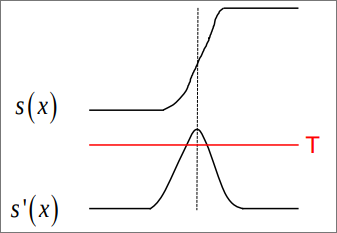
\includegraphics[width=0.45\textwidth]{1dstepedge}
    \end{center}
    \label{fig:1dstep}
\end{figure}
Accordingly, the simplest edge-detection operator relies on thresholding the absolute value of the first derivative of the signal. 
\subsection{2D Step-Edge} % step-edge, I'm stuck!
A 2D Step-Edge is characterized by both strength and direction. Hence, we cannot use a directional derivative but instead we need an operator allowing to sense the edge whatever its direction is. For this purpose, we use the gradient:
\[
    \nabla I(x,y)=\displaystyle\frac{\partial I (x,y)}{\partial x}i + \displaystyle\frac{\partial I (x,y)}{\partial y} j
\]
The direction of the gradient is that of the highest variation of the function, while its magnitude is the absolute value of the directional derivative along such direction. 

\subsection{Edge detection by Gradient Thresholding}
\begin{figure}[!ht]
    \begin{center}
        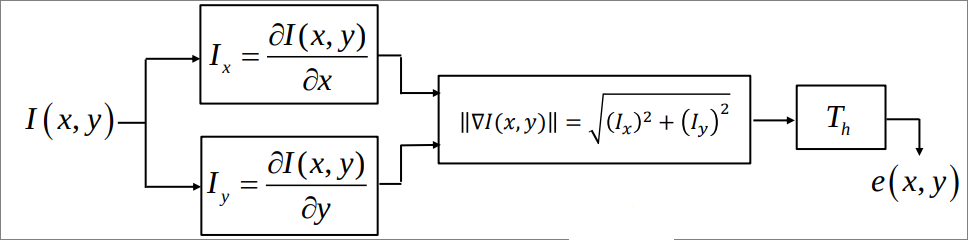
\includegraphics[width=0.95\textwidth]{edging}
    \end{center}
    \label{fig:edging}
\end{figure}

Edge detection by gradient thresholding can be achieved by applying this scheme 
\subsubsection{Discrete approximation of the gradient}
Backward or forward differences can be used:
\begin{gather*}
    \displaystyle\frac{\partial I(x,y)}{\partial x} \cong I_x(i,j)=I(i,j)-I(i,j-1), \quad     \displaystyle\frac{\partial I(x,y)}{\partial y} \cong I_y(i,j)=I(i,j)-I(i-1,j)\\
    \displaystyle\frac{\partial I(x,y)}{\partial x} \cong I_x(i,j)=I(i,j)-I(i,j+1), \quad     \displaystyle\frac{\partial I(x,y)}{\partial y} \cong I_y(i,j)=I(i,j)-I(i+1,j)
\end{gather*}
which may be thought of as correlation by:
\[
    \begin{bmatrix}
        -1 & 1
    \end{bmatrix}\quad
    \begin{bmatrix}
        -1 \\ 1
    \end{bmatrix}
\]
Or also central differences:
\[
    \displaystyle\frac{\partial I(x,y)}{\partial x} \cong I_x(i,j)=I(i,j+1)-I(i,j-1), \quad     \displaystyle\frac{\partial I(x,y)}{\partial y} \cong I_y(i,j)=I(i+1,j)-I(i-1,j)\\
\]
with the corresponding correlation kernels given by:
\[
    \begin{bmatrix}
        -1 & 0 & 1
    \end{bmatrix}\quad
    \begin{bmatrix}
        -1 \\ 0 \\ 1
    \end{bmatrix}
\]
We can estimate the magintude by different approximations:
\begin{align*}
    \|\nabla I\|_2&=\sqrt{I_x^2+I_y^2} \\ \|\nabla I \|_1 &= |I_x| + |I_y| \\ \|\nabla I \|_\infty &= max(I_x,I_y) \end{align*}
The third approximation is faster and more invariant wrt edge direction. 

However, it is well known that differetiation amplifies noise, making edge detection through differentiation problematic. It is therefore necessary to denoise images for edge detection, which does however lead to blurred edges that will be harder to detect. 
\subsection{Smooth Derivatives}
Smoothing and differentiation are carried out jointly within a single step. This is achieved  by computing differences of means. To avoid blurring edges, the two operations are carried out along orthogonal directions
\begin{gather*}
    \mu_x(i,j)=\displaystyle\frac{1}{3}[I(i,j-1)+I(i,j)+I(i,j+1)] \quad \mu_y(i,j)=\displaystyle\frac{1}{3}[I(i-1,j)+I(i,j)+I(i+1,j)]\\
    \tilde{I}_x(i,j) = \mu_y(i,j+1)-\mu_y(i,j) =\\= \displaystyle\frac{1}{3}[I(i-1,j+1)+I(i,j+1)+I(i+1,j+1)-I(i-1,j)-I(i,j)-I(i+1,j)]\\
    \implies \text{ which is equivalent to the kernel }\displaystyle\frac{1}{3}\begin{bmatrix}
        -1 & 1 \\
        -1 & 1 \\
        -1 & 1 
    \end{bmatrix}
\end{gather*}
and similarlty for $\tilde{I}_y(i,j)$ the kernel turns out to be:
\[
    \displaystyle\frac{1}{3}\begin{bmatrix}
        -1 & -1 & -1 \\
        1 & 1 & 1
    \end{bmatrix}
\]
In the \emph{Prewitt operator}, derivatives are approximated by central differences (better for diagonal edges)
\begin{gather*}
    \tilde{I}_x(i,j)=\mu_y(i,j+1)-\mu_y(i,j-1) \quad \implies \quad \frac{1}{3} \begin{bmatrix}
        -1 & 0 & 1 \\
        -1 & 0 & 1 \\
        -1 & 0 & 1 
    \end{bmatrix}\\
    \tilde{I}_y(i,j)=\mu_x(i,j+1)-\mu_x(i,j-1) \quad \implies \quad \frac{1}{3} \begin{bmatrix}
        -1 & -1 & -1 \\
        0 & 0 & 0 \\
        1 & 1 & 1 
    \end{bmatrix}
\end{gather*}
In the \emph{Sobel operator}, the central pixel is weighted more to further improve isotropy:
\begin{gather*}
    \mu_y(i,j)=\displaystyle\frac{1}{4}[I(i-1,j)+2(i,j)+I(i+1,j)]\\
    \tilde{I}_x(i,j)= \mu_y(i,j+1)-\mu_y(i,j-1)\\
    \implies \displaystyle\frac{1}{4}\begin{bmatrix}
        -1 & 0 & 1 \\
        -2 & 0 & 2 \\
        -1 & 0 & 1 \\
    \end{bmatrix}
\end{gather*}
Thresholding is suboptimal for edge localization, therefore we search for maxima of the gradient magnitude. 
\subsection{Non maxima suppression}
Maxima are searched along the gradient direction. Pixels that are not maxima are suppressed
\subsubsection{Discrete formulation}
The gradient direction is discretized. 2$\pi$ is divided into 8 direction bins 
\subsubsection{Continuous formulation}
Is based on gradient interpolation

The overall flow-chart of an edge detector based on smooth derivatives and NMS can be sketched as in the figure 
\begin{figure}[!ht]
    \begin{center}
        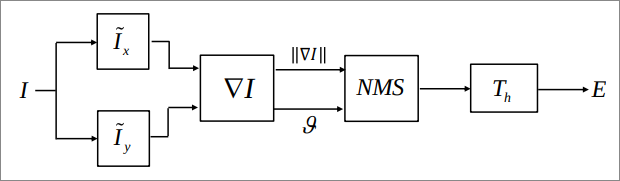
\includegraphics[width=0.95\textwidth]{smoothedging}
    \end{center}
    \label{fig:sedge}
\end{figure}

\subsection{Canny's Edge Detector}
Canny proposed a set of criteria to evaluate an edge detector:
\begin{enumerate}
    \item Good detection: robustness to noise
    \item Good localization: edges should be localized with the minimum possible error (distance to the "true" edge)
    \item One response to one edge: the filter should detect one single edge point at each "true" edge
\end{enumerate}
In the 1D case, the optimal edge detection consists in finding local extrema of the convolution of the signal by a 1st order Gaussian derivative (Gaussian: smoothing, derivative: variations). This theoretical result can also be regarded as proof that the gaussian filter is optimal for smoothing to detect noisy edges.

In the 2D case, the optimal filter results to be composed of the sequence of Gaussian smoothing, gradient computation and NMS along the gradient direction. 
2D convolution by a gaussian can be sped up through separability:
\begin{gather*}
    \tilde{I}_x(x,y) = \frac{\partial}{\partial x} (I(x,y)\ast G(x,y)) = I(x,y) \ast \frac{\partial G(x,y)}{\partial x}\\
    \tilde{I}_y(x,y) = \frac{\partial}{\partial y} (I(x,y)\ast G(x,y)) = I(x,y) \ast \frac{\partial G(x,y)}{\partial y}\\
    G(x,y) = G(x)G(y)\\
    \Downarrow\\
    \tilde{I}_x(x,y) = I(x,y) \ast (G'(x)G(y))  =(I(x,y)\ast G'(x))\ast G(y)\\
    \tilde{I}_x(x,y) = I(x,y) \ast (G'(x)G(y))=(I(x,y)\ast G'(x))\ast G(y)
\end{gather*}
After NMS an extra thresholding is applied to distinguish true edges and unwanted ones. However, edge streaking may occur when gradient magnitude varies along object contours. To address this issue, Canny proposed \emph{hysteresis thresholding}: 2 thresholds are used, a higher ($T_h$) and a lower ($T_l$) one. Pixels are taken as an edge if they are above $T_h$ or if they are higher than $T_l$ and are neighbours to an already detected edge. The overall flow-chart of the Canny edge detector is as follows:
\begin{figure}[!ht]
    \begin{center}
        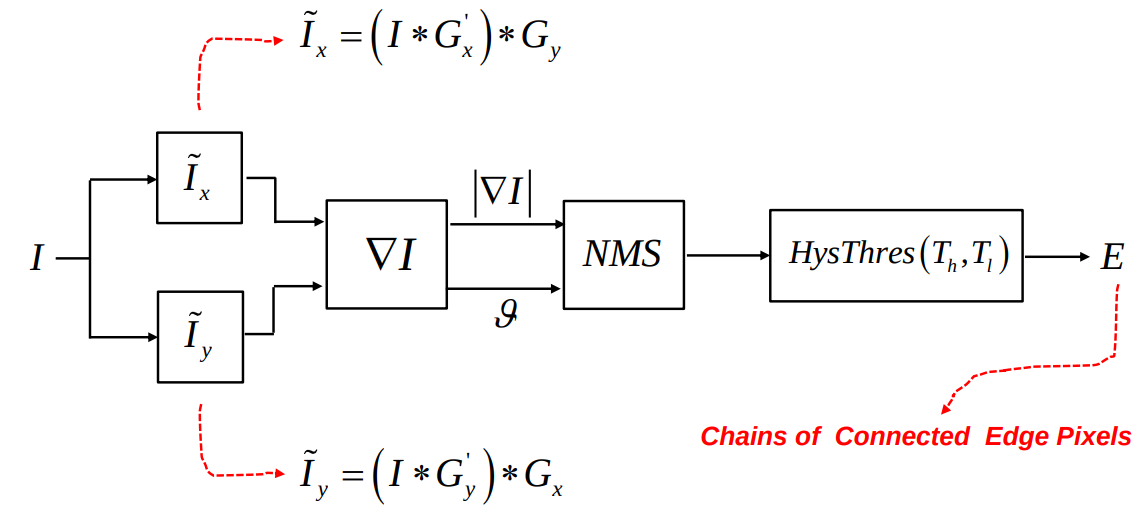
\includegraphics[width=0.95\textwidth]{canny}
    \end{center}
    \label{fig:canny}
\end{figure}

\subsection{Edge detection through the second derivative}
Edges may also be located by looking for zero-crossing of the second derivative of the signal. The second derivative along the gradient direction can be obtained as $n^THn$ where 
\[
    n = \frac{\nabla I(x,y)}{\|\nabla I(x,y)\|} \quad \text{and} \quad H = \begin{bmatrix}
        \frac{\partial^2I(x,y)}{\partial x^2} & \frac{\partial^2I(x,y)}{\partial x \partial y}\\
        \frac{\partial^2I(x,y)}{\partial y \partial x} & \frac{\partial^2I(x,y)}{\partial y^2}
    \end{bmatrix}
\]
Computing this turns out to be very slow, so instead we can rely on the Laplacian as a second order differential operator 
\[
    \nabla^2 I(x,y) = \frac{\partial^2I(x,y)}{\partial x^2}+\frac{\partial^2I(x,y)}{\partial y^2} = I_{xx}+I_{yy}
\]
\subsubsection{Discrete Laplacian}
One can use forward and backward differences to approximate the first and second order derivatives respectively:
\[
    I_{xx} \simeq I_x(i,j)-I_x(i,j-1)=I(i,j-1) - 2I(i,j)+I(i,j+1)
\]
$I_{yy}$ analogous. This leads to the following convolution kernel:
\[
    \nabla^2 = \begin{bmatrix}
        0 & 1  & 0 \\
        1 & -4  & 1 \\
        0 & 1  & 0 
    \end{bmatrix}
\]
It can be shown that the zero-crossing of the Laplacian typically lies close to those of the second order derivative along the gradient, while being much faster to compute. 
\subsubsection{Laplacian of Gaussian (LOG)}
Gaussian smoothing is deployed along edge detection through the Laplacian, forming an edge detector referred to as LOG (Laplacian of Gaussian). Edge detection by the LOG can be summarized conceptually as:
\begin{enumerate}
    \item Gaussian smoothing: $\tilde{I}(x,y) = I(x,y) \ast G(x,y)$ 
    \item Second order differentiation by the Laplacian: $\nabla^2\tilde{I}(x,y)$
    \item Extraction of the zero-crossing of $\nabla^2\tilde{I}(x,y)$ 
\end{enumerate}
\section{Finding Correspondences between images}
A great variety of computer vision problems can be dealt with by finding \emph{corresponding points} betweeen two or more images of a scene. The task of establishing correspondences is split into 3 successive steps: 
\begin{enumerate}
    \item Detection of salient points
    \item Description - computation of a suitable descriptor based on a neighbourhood around a key point 
    \item Matching descriptors between images
\end{enumerate}
and should be invariant to the transformations that may relate images. 
\subsection{Properties of good detectors/descriptors}

\begin{itemize}
  \item Detector \begin{itemize}
      \item Repeatablity: finding the same salient points in different images 
      \item Saliency: finding useful points 
    \end{itemize}
  \item Descriptor \begin{itemize}
      \item Distinctiveness vs robustness trade-off
      \item Compactness: descriptions should be concise
    \end{itemize}
\end{itemize}
Good keypoints should exhibit a large variation along all directions. 
\subsection{Moravec Corner Detector}
\[
  C(p) = \min_{q\in n_8(p)} \|N(p)-N(q)\|^2 
\]
The cornerness at $p$ is given by the minimum squared difference between the values of the pixels in the patch centered at $p$ and those centered at its 8 neighbours. The cornerness of the whole image is computed, then thresholding and NMS are applied to identify corners.
\subsection{Harris Corner Detector}
The Harris corner detector is a continuous formulation of the Moravec corner detector. Denoting as $(\Delta x,\Delta y)$ a generic infinitesimal shift, the error function may be written as:
\begin{align*}
  E(\Delta x, \Delta y ) = \displaystyle\sum_{x,y}^{}w(x,y)(I(x+\Delta x, y + \Delta y)-I(x,y))^2
\end{align*}
Where $w(t)$ is $1$ inside the chosen neighbourhood and $0$ elsewhere.
Due to the shift being infinitesimal, we may take advantage of Taylor series expansion of the intensity function at $(x,y)$:
\[
  I(x+\Delta x, y+ \Delta y)-I(x,y) \simeq \displaystyle\frac{\partial I(x,y)}{\partial x}\Delta x + \displaystyle\frac{\partial I(x,y)}{\partial y}\Delta y = I_x(x,y)\Delta x + I_y (x,y) \Delta y
\]
\begin{align*}
    E(\Delta x, \Delta y ) &= \displaystyle\sum_{x,y}^{}w(x,y)(I_x(x,y)\Delta x + I_y(x,y)\Delta y )^2\\
    &=  \displaystyle\sum_{x,y}^{}w(x,y)(I_x(x,y)^2\Delta x^2 + I_y(x,y)^2\Delta y^2 + 2I_x(x,y)I_y(x,y)\Delta x \Delta y )\\
    &=\displaystyle\sum_{x,y}^{}w(x,y)\left( \begin{bmatrix}
      \Delta x \Delta y
      \end{bmatrix} \begin{pmatrix}
      I_x^2 & I_xI_y \\
      I_yI_x & I_y^2
      \end{pmatrix} \begin{bmatrix}
      \Delta x \\ \Delta y
  \end{bmatrix}\right) \\
    E(\Delta x, \Delta y) &= \begin{bmatrix}
    \Delta x & \Delta y
    \end{bmatrix} M \begin{bmatrix}
    \Delta x \\ \Delta y
  \end{bmatrix}
\end{align*}
where
\[
    M = (\nabla I)^\top\nabla I
\]
wlog we can assume $M$ to be diagonal, as it is real and symmetric, thus always diagonalizable:
\[
  M=\begin{pmatrix}
    \lambda_1 & 0 \\ 0 & \lambda_2
  \end{pmatrix} \implies E(\Delta x, \Delta y) = \lambda_1 \Delta x^2 + \lambda_2 \Delta y^2
\]
we have that if: 
\begin{itemize}
  \item $\lambda_1, \lambda_2 \simeq 0$: we are in a flat region 
  \item $\lambda_1 >> \lambda_2 $: we are on an edge
  \item $\lambda_1, \lambda_2 >> 0$: we are in a corner
\end{itemize}
The previous considerations also hold with $M$ not diagonal by diagonalization:
\[
  M = R \begin{pmatrix}
    \lambda_1 & 0 \\ 0 & \lambda_2
  \end{pmatrix} R^T
\]
where the columns of $R$ are the orthonormal eigenvectors of $M$, and  $R^T$ is the rotation matrix that aligns the image axes to the eigenvectors of M.
Computing the eigenvalues of $M$ may be slow, thus a more efficient cornereness function is proposed: 
\[
  C= det(M)-k \cdot tr(M)^2 = \lambda_1\lambda_2 -k (\lambda_1+\lambda_2)^2
\]
With this new function we have 
\begin{itemize}
  \item $C \simeq 0$: Flat region
  \item $C > 0$: Corner
  \item $C < 0$: Edge
\end{itemize}
It is worth noting that the weighing function used is actually not a box function but rather Guassian shaped to assign more weight to closer pixels. Corner detection follows the same steps as with the Moravec corner detector:
\begin{itemize}
  \item computing the cornerness $C$ 
  \item Thresholding the values of $C$ 
  \item perform NMS on the thresholded values of $C$
\end{itemize}



\subsection{Shi-Tomasi Corner Detector}
A popular variant to the Harris corner detector, providing better results when tracking corner points across  video frames. The cornerness function is:
\[
  C=\min(\lambda_1,\lambda_2)
\]
Where $\lambda_1, \lambda_2$ are as defined above for the Harris corner detector.
It results particularly useful in tracking corner points in videos. 
\subsection{Invariance properties of the Harris corner detector}
\subsubsection{Rotation}
Yes, as the eignevalues of matrix $M$ are invariant to rotation of the image axes
\subsubsection{Intensity changes}
\begin{itemize}
  \item yes, to additive bias $(I'=I+b)$ due to the use of derivatives
    \item no to a linear change $(I' = aI)$ as derivatives undergo the same change
\end{itemize}
so overall, no invariance to affine intensity changes. 
\subsubsection{Scale}
No, due to fixed detection window size (impossible to detect homologous features when they appear at different scales in images - e.g. a corner at some scale might appear as an edge at another scale). Images contain features at different scales, thus a multiscale feature detector is necessary. A point may show up as salient at different scales. The \emph{characteristic scale} of a feature is the scale at which it's more salient. In order to match descriptors, large scale features need to be smoothed in order to eliminate details that do not appear across the range of scales. A fixed size detection tool is used on increasingly down-sampled and smoothed versions of the input image. 

\section{Scale-Space}
A Scale-Space is a one-parameter family of images created from the original so that the structures at smaller scales are successively suppressed by smoothing operations. Moreover, the scale-space should not introduce artifacts. From studies it has been shown that Gaussian smoothing is the only viable solution: 
\[
  L(x,y,\sigma) = G(x,y,\sigma)\ast I (x,y)
\]
Thus, a scale-space is created by repeatedly smoothing with larger and larger Gaussian kernels, or equivalently, by solving a 2D diffusion PDE over time starting from the original image: 
\[
  \frac{\partial I(x,y,t) }{\partial t} = k\nabla^2I(x,y,t) \implies \sigma=\sqrt{2kt}
\]
In order to detect features and select their characteristic scale, we can find the extrema of certain combinations of scale-normalized derivatives of the Guassian Scale-Space. The method consists in stacking the chosen Gaussian derivatives and seeking for extrema along space and scale. As we smooth more (i.e., larger $\sigma$), derivatives become weaker, thus they are multiplied by $\sigma^2$ to normalize them.
\subsection{Scale-normalized LOG}
One proposed combination of derivatives is the Laplacian of Gaussian.
\[
    F(x,y,\sigma) = \sigma^2\nabla^2L(x,y,\sigma) = \sigma^2(\nabla^2 G(x,y,\sigma)\ast I(x,y))
\]
blob-like features and scales are detected as extrema of the scale-normalized LOG.
\subsection{DoG Detector}
\[
    DoG(x,y,\sigma) = (G(x,y,k\sigma)-G(x,y,\sigma))\ast I(x,y) = L(x,y,k\sigma)-L(x,y,\sigma)
\]
This approach provides a computationally efficient approximation of the scale-normalized LOG:
\[
    G(x,y,k\sigma)-G(x,y,\sigma)\approx (k-1)\sigma^2\Delta^2 G(x,y,\sigma)
\]
as $(k-1)$ is constant, it does not influence the location of extrema. As such, the choice of $k$ is not critical. The DoG detector is rotation invariant.
\subsubsection{Computation of DoG}
In general, in an octave, $s$ DoG images are computed (octave: interval from $n\sigma$ to $2n\sigma$). Rather than doubling $\sigma$ for the filters of the next octave, we downsample $L(x,y,2\sigma)$ by taking half of the columns and rows and then use the same filters.

A point is detected as a maximum if the DoG is higher than the $n_8$ neighbourhood in the same image and in the images above and below ($8+9+9=26$ neighbours) (3D NMS)

\subsection{Scale and rotation invariant description}
\begin{itemize}
    \item Most keypoint detection algorithms rely on finding extrema across a stack of images computed while increasing a scale parameter 
    \item Then, once each keypoint has been extracted, the surrounding patch is considered to compute its descriptor. A desirable property concerns such descriptor being scale and rotation invariant.
    \item To attain scale invariance, the patch is taken from the stack image ($L(x,y,\sigma$) that corresponds to its carachteristic scale. As such, the descriptor is computed on a smooth patch that does not contain fine details that are not preserved across the range of scales
    \item To attain rotation invariance, a canonical patch orientation is computed, so that the descriptor can then be computed on a canonically-oriented patch
\end{itemize}

\subsection{Canonical orientation}
A reasonable choice is the direction along which most of the gradient is found. It is used to define a local reference frame for image patches. Gradient magnitude and orientation are computed at each pixel of the patch, then an orientation histogram with bin size $10^\circ$ is created by accumulating the contributions of the pixels belonging to a neighbourhood of the keypoint location. The contribution of each pixel to its designated orientation bin is given by the gradient magnitude weighted by a Gaussian with $\sigma = 1.5\sigma_s$ where $\sigma_s$ is the scale of the keypoint. The canonical orientation is taken as the peak of the histogram, with parabola interpolation of the histogram around the peak using the two columns adjacent to the peak. Other peaks higher than 0.8 of the main one would be kept as well, yielding multiple canonical orientations and thus descriptors sharing the same location/scale with diverse orientations. This has been found to occur quite rarely.

\section{Sift Descriptor}
The SIFT descriptor is computed as follows: 
\begin{itemize}
    \item A 16x16 pixel grid around each keypoint is considered.
    \item This grid is divided into 16 4x4 pixel subgrids.
    \item For each subgrid, the gradient magnitude and orientation are computed for each pixel and a gradient orientation histogram is built with 8 bins.
    \item Gradients are rotated according to the canonical orientation of the keypoint.
    \item Each pixel in the region contributes to its designated bin according to gradient magnitude as well as to a Gaussian weighting function with $\sigma$ equal to half the grid size. 
    \item To avoid boundary effects, a soft assignment is employed: each pixels contribution to two adjacent bins is weighted by the distance to the bin center. This is done within a histogram and also between regions. The overall scheme is referred to as trilinear interpolation. 
    \item The descriptor is normalized to unit length to gain invariance wrt affine intensity changes. Then to increase robustness to nonlinear changes, all elements larger than 0.2 are saturated and the descriptor is normalized again.
\end{itemize}

\section{Matching process}
The most widely used method to compare descriptors is to compute the euclidean distance between descriptors. This gives rise to a nearest neighbour search problem: given a set $S$ of points $p_i$ in a metric space $M$ and a query point $q$, find $p_i\in S$ closest to $q$.

The found NN could be a bad match, therefore there are some criteria to accept or reject a match:
\begin{itemize}
    \item $d_{NN}\leq T$ (NN distance) 
    \item $\displaystyle\frac{d_{NN}}{d_{2-NN}} \leq T$ (ratio of distances)
\end{itemize}
For the NN distance criterion, it is hard to pick a threshold. Lowe shows that for ratio of distances criterion $T=0.8$ may allow to reject 90\% of false matches while only missing 5\% of correct ones.

\subsection{Efficient NN search}
Brute force search is not efficient, as it requires $O(N)$ operations. A more efficient approach is to use a data structure that allows for fast search. A common choice is the k-d tree, which is a binary tree that splits the space into half-spaces. The preferred approach is the \emph{approximate} variant referred to as \emph{BBF (Best Bin First)}. This formulation is efficient also in high-dimensional spaces such as descritpor spaces ($\R^{128}$ for SIFT).

\subsubsection{k-d tree}
Construction:
\begin{enumerate}
    \item Start with a list of $k$-dimensional points 
    \item At each level: 
        \begin{itemize}
            \item select a dimension to split the data 
            \item sort the points along that dimension 
            \item choose the median point as the root
        \end{itemize} 
    \item Recursively repeat for the left and right subsets:
        \begin{itemize}
            \item Left: all points smaller than the median along the splitting dimension 
            \item Right: all points greater than or equal to the median along the splitting dimension
        \end{itemize}
\end{enumerate}
NN search:
\begin{enumerate}
    \item given the query $q$, the tree is traversed from root to the closest leaf, denoted as $NN_{curr}$ with distance $d(q,NN_{curr})$ from $q$. 
    \item Backtracking:
        \begin{enumerate}
            \item the parent node to the found leaf is considered: if its distance to $q$ is less than $d(q,NN_{curr})$ the parent node becomes the new $NN_{curr}$ and $d(q,NN_{curr})$ is updated. 
            \item A check is carried out to determine whether the other half-space defined by the current parent node may contain or not a closer point. This depends on whether or not the hypersphere of radius $d(q,NN_{curr})$ centered at $q$ does intersect the splitting hyperplane.
                \begin{itemize}
                    \item In the first case, the sub-tree whose root is the parent node is traverse down to the next closest leaf 
                    \item Conversely, the parent node to the current one is considered.
                \end{itemize}
            \item The process ends upon getting to the root of the tree, with $NN_{curr}$ being the nearest neighbour to $q$.
        \end{enumerate}
\end{enumerate}
Best Bin First search:
\begin{enumerate}
    \item given the query $q$, the tree is traversed from root to the closest leaf, denoted as $NN_{curr}$ with distance $d(q,NN_{curr})$ from $q$. The visited nodes are ordered in a \emph{priority queue} according to their distance to $q$. 
    \item Backtracking:
        \begin{enumerate}
            \item The first element in the \emph{priority queue} is extracted so to traverse its unexplored branch down to a leaf. During the process, the priority queue is kept updated. 
            \item The previous step is iterated until a fixed number of leaves ($E_{max}$) have been visited.
        \end{enumerate}
\end{enumerate}
The found \emph{approximate} NN is the closest data point $NN_{curr}$ after $E_{max}$ leaves have been visited.

\section{Instance Detection}
Detection of a specific instance of an object in an image. Given a reference image of a specific object, the task is to determine whether it is present or not in the image under analysis.

\subsection{Template matching}
The model image is slid across the target image to compare it with a same size window with a (dis)similarity function.
\subsubsection{Dis(similarity) functions}
\begin{itemize}
    \item   Sum of squared differences (SSD):
        \[
            SSD(i,j) = \displaystyle\sum_{m=0}^{M-1}\displaystyle\sum_{n=0}^{N-1}(I(i+m,j+n)-T(m,n))^2
        \]
        both $\tilde{I}(i,j)$ (i.e., the window fo the target image at position $(i,j)$ having the same size as $T$) and $T$ can be though of as $M\cdot N$-dimensional vectors through flattening. Accordingly, $SSD$ represents the squared L2 norm of their difference.
    \item Sum of Absloute Differences (SAD):
        \[
            SAD(i,j) = \displaystyle\sum_{m=0}^{M-1}\displaystyle\sum_{n=0}^{N-1}|I(i+m,j+n)-T(m,n)|
        \]
        which is the L1 norm of the difference between the two vectors.
    \item Normalized Cross-Correlation (NCC):
        \[
            NCC(i,j) = \displaystyle\frac{\displaystyle\sum_{m=0}^{M-1}\displaystyle\sum_{n=0}^{N-1}I(i+m,j+n)\cdot T(m,n)}{\sqrt{\displaystyle\sum_{m=0}^{M-1}\displaystyle\sum_{n=0}^{N-1}I(i+m,j+n)^2 \cdot \displaystyle\sum_{m=0}^{M-1}\displaystyle\sum_{n=0}^{N-1}T(m,n)^2}}
        \]
        \[
            NCC(i,j) = \displaystyle\frac{\tilde{I}(i,j)\cdot T}{\|\tilde{I}(i,j)\|\cdot \|T\|} = \displaystyle\frac{\|\tilde{I}(i,j)\|\cdot \|T\|\cdot \cos\theta}{\|\tilde{I}(i,j)\|\cdot \|T\|} = \cos\theta \quad \implies \quad \tilde{I}(i,j) 0 \alpha \cdot T 
        \]
        thus $NCC$ represents the cosine of the angle betwen vectors $\tilde{I}(i,j)$ and $T$ and is therefore invariant to linear intensity changes.
        \item Zero-mean Normalized Cross-Correlation (ZNCC):
            \[
                ZNCC(i,j) = \displaystyle\frac{\displaystyle\sum_{m=0}^{M-1}\displaystyle\sum_{n=0}^{N-1}(I(i+m,j+n)-\mu_{\tilde{I}})(T(m,n)-\mu_T)}{\sqrt{\displaystyle\sum_{m=0}^{M-1}\displaystyle\sum_{n=0}^{N-1}(I(i+m,j+n)-\mu_{\tilde{I}})^2 \cdot \displaystyle\sum_{m=0}^{M-1}\displaystyle\sum_{n=0}^{N-1}(T(m,n)-\mu_T)^2}}
            \]
            where $\mu_{\tilde{I}}$ and $\mu_T$ are the means of the target and template windows respectively.
            $\tilde{I}(i,j) = \alpha\cdot T + \beta$, thus $ZNCC$ is invariant to affine intensity changes.
\end{itemize}
\subsubsection{Fast template matching}
Template matching may turn out exceedingly slow when the model and/or target images have a large size ($O(M\times N \times W \times H)$). The simplest approach to speed-up computation is to deploy an \emph{image pyramid}:
\begin{itemize}
    \item smoothing and subsampling both model and target image (typically by a factor of 2 on both sides per level) 
    \item Full search at top level and then local refinements traversing back the pyramid down to the original image 
    \item To handle rotation and/or scale changes on would need to probe rotated and/or scaled model images, possibly while deploying an image pyramid to speed up the process
\end{itemize}

\subsection{Shape-based matching}
May be thought of as an edge-based template matching. First, a set of control points $P_k$ is extracted form the model image by an edge detection operation (e.g. Sobel) and the gradient direction at each $P_k$ is recorded. 
Then, at each position $(i,j)$ of the sliding window within the target image, the recorded gradient directions associated with control points are compared to those at their corresponding image points $\tilde{P}_k(i,j)$ in order to compute a similarity function.
\begin{align*}
    &G_k(P_k) = \begin{bmatrix}
        I_x(P_k) \\ I_y(P_k)
    \end{bmatrix}, \quad u_k(P_k) = \displaystyle\frac{1}{\|G_k(P_k)\|}G_k(P_k), \quad k=1,\dots,n\\ 
    &\tilde{G}_k(\tilde{P}_k) = \begin{bmatrix}
        I_x(\tilde{P}_k) \\ I_y(\tilde{P}_k)
    \end{bmatrix} \quad \tilde{u}_k(\tilde{P}_k) = \displaystyle\frac{1}{\|\tilde{G}_k(\tilde{P}_k)\|}\tilde{G}_k(\tilde{P}_k), \quad k=1,\dots,n\\
    &S(i,j) = \displaystyle\frac{1}{n} \displaystyle\sum_{k=1}^{n}u_k(P_k)^\top \tilde{u}_k(\tilde{P}_k) = \displaystyle\frac{1}{n} \displaystyle\sum_{k=1}^{n}\cos(\theta_k)
\end{align*}
The above similarity function spans the interval $[-1,1]$, taking maximum value when all the gradients at the control points in the current window of the target image are perfectly aligned to those at the control points of the model image. Choosing a detection threshold can be thought of as specifying the fraction of model points which must be seen in the image to trigger a detection.

To achieve invariance to contrast polarity changes, the following modification is possible:
\[
    S(i,j) \displaystyle\frac{1}{n} \left|\displaystyle\sum_{k=1}^{n}u_k(P_k)^\top \tilde{u}_k(\tilde{P}_k) \right| = \displaystyle\frac{1}{n} \left|\displaystyle\sum_{k=1}^{n}\cos(\theta_k)\right|
\]
This achieves invariance to global inversions of contrast polarity along object contours. To acheive invariance to local inversions, the following modification is possible:
\[
    S(i,j) = \displaystyle\frac{1}{n} \displaystyle\sum_{k=1}^{n}\left|u_k(P_k)^\top \tilde{u}_k(\tilde{P}_k) \right| = \displaystyle\frac{1}{n} \displaystyle\sum_{k=1}^{n}\left|\cos(\theta_k)\right|
\]
Edges in the target image are not computed as the control points are extracted from the model image. Thus, this method is robust to the fragility of edge detection given  by light changes.
\subsection{The Hough Transform}
The Hough Transform enables to detect objects having a shape that can be expressed by an equation, based on projection of the input data into a suitable space referred to as \emph{parameter} or \emph{Hough} space. Typically the HT is applied after an edge detection process, i.e. the input data consists of the edge pixels extracted from the original image. 
The HT is robust to noise and allows for detecting the sought shape even thoug it is partially occluded in the image.
\subsubsection{Line detection}
let us consider the equation of a line:
\[
    y-mx-c = 0
\]
In the usual image space interpretation of the line equation, the parameters $\hat{m}$ and $\hat{c}$ are fixed:
\[
    y-\hat{m}x-\hat{c} = 0
\]
so that the equation represents a mapping from point $\hat{m}, \hat{c}$ of the parameter space to the image points belonging to the line. We may instead fix $\hat{x}, \hat{y}$:
\[
    \hat{y}-m\hat{x}-c = 0
\] 
so that the equation represents a mapping from point $\hat{x}, \hat{y}$ of the image space to the lines passing through the point. Such a locus is itself a line. 

Accordingly, if we consider to image points $P_1, P_2$ and map both to into the parameter space, we get two lines intersecting at the parameter space point represneting the image line through $P_1, P_2$. Thus, for $n$ collinear image points the line parameters $(m,c)$ are identified by the single intersection of $n$ lines in the parameter space. In looking for a line in the image space we therefore look for a point that is an intersection of lines in the parameter space. More in general, given a sought analytic shape represented by a set of parameters, the HT consists in mapping image points (usually edge points) so as to create curves into the parameter space of the shape, the intersections of which indicate the presence of image points explained by a certain instance of the shape, with more curve intersecting indicating stronger support for presence of the shape in the image.

In practice, to make the process work, the parameter space is discretized and allocated as a memory array, which is typically referred to as Accumulator Array (AA). Then, curves are drawn into the AA by a so called \emph{voting} process: the tranform equation si epeatedly computed to increment the bins satisfying the equation. Accordingly, a high number of intersecting curves at a point of the parameter space will provide a high number of votes into a bin of the AA. Finding parameter space points through which many lines intersect is thus implemented by finding peaks of the AA, i.e. local maxima showing a high number of votes (NMS).

The usual line parametrization is impractical for the HT, as vertical lines would require infinite values of $m$ and $c$. A more suitable parametrization is the \emph{normal parametrization}: 
\[
    \rho = x\cos\theta + y\sin\theta
\]
Image points are mapped into sinusoidal curves of the $(\theta, \rho)$ parameter space. With the normal parametrization, $\theta\in\left[-\displaystyle\frac{\pi}{2}, \displaystyle\frac{\pi}{2}\right]$, $\rho\in \left[-\rho_{max},\rho_{max}\right]$, where $\rho_{max}$ is usually taken as large as the image diagonal. 

\subsubsection{Circle detection}
The equation of a circle is:
\[
    (x-a)^2+(y-b)^2 = r^2
\]
Through the HT this is interpreted as a mapping from the image space to the 3-dimensional parameter space $(a,b,r)$. The points satisfying the equation of the circle lie on a cone in the Hough space, with its axis parallel to the $r$ axis. A 3D AA may be implemented, with each layer being associated to a value of $r$:
\[
    \forall \bar{r} \in [r_{min}, r_{max}]: \quad \begin{cases}
        a = \hat{x} + \bar{r}\cos\theta_k\\
        a = \hat{y} + \bar{r}\sin\theta_k
    \end{cases} \qquad \theta_k \in \left[0,2\pi\right] \quad \begin{cases}
        \Delta \theta = \displaystyle\frac{2\pi}{M}\\
        \theta_k = k\Delta \theta, \ k=0,\dots,M
    \end{cases}
\]
\subsection{Generalized Hough Transform}
The HT can be extended to detect arbitrary non analytical shapes. A description of the algorithm follows:
\begin{itemize}
    \item \textbf{Off-line Phase}
        \begin{enumerate}
            \item Detect edges (B) in the model image
            \item Choose a reference point $y$ (e.g. the barycenter of B) 
            \item For each point $x$ in $B$:
                \begin{enumerate}
                    \item Compute vector $r$ from $x$ to $y$ (i.e. $r=y-x$) 
                    \item Compute the direction of the gradient at $x$ $\varphi(x)$ 
                    \item Store $r$ in a table (R-table) indexed by a chosen gradient direction quantization step $\Delta\varphi$
                \end{enumerate}
        \end{enumerate} 
    \item \textbf{On-line Phase (object detection)} 
    \begin{enumerate}
        \item Detect edges in teh target image and initialize another iamage as accumulater array $A[y]$. For eachg edge pixel $x$ of the target image:
        \item Compute gradient direction $\varphi$ at $x$ 
        \item Quantize $\varphi$ to index the R-table. For each $r_i$ vector stored in the indexed row:
            \begin{enumerate}
                \item Compute the position of the reference point $y=x-r_i$ 
                \item Cast a vote into the accumulator array $A[y]++$ 
            \end{enumerate}
        \item As usual with the HT, instances of the sought object are detected by finding peaks in the accumulator array.
    \end{enumerate}
\end{itemize}
\subsubsection{Invariance to rotation and scale}
To gain invariance from rotation, it is necessary to quantize the rotation range and try al possible discretized rotations (brute force approach). This is only feasible for small rotation ranges
\[
    \forall r:y=x+r_\theta =x + ROT(r,\theta), \quad A[y,\theta]++
\]
To handle scale changes a similar approach needs to be taken:
\[
    \forall r:y=x+r_s = x + s\cdot r, \quad A[y,s]++
\]
Handling rotation and scale (similarity) requires that both approaches be taken together:
\[
    \forall r:y=x+ s\cdot r_\theta, \quad A[y,\theta,s]++
\]
This is hardly feasible
\subsection{GHT with Local Invariant Features aka Star Model}
\textbf{Off-line}:
\begin{enumerate}
    \item Detect keypoints (e.g. DoG) and compute descriptors (e.g. SIFT) in the model image:
        \[
            F =\{ F_1, F_2,\dots F_N \} \qquad F_i = (P_i, D_i, \varphi_i, S_i)
        \]
        where $P_i$ is the keypoint position, $D_i$ is the descriptor, $\varphi_i$ is the orientation and $S_i$ is the scale. 
    \item Choose a reference point (e.g. barycenter of $P_i$)
        \[
            P_C = \displaystyle\frac{1}{N}\displaystyle\sum_{i=1}^{N}P_i
        \] 
        \item Compute the joining vectors between the features and the reference point:
            \[
                \forall F_i \in F \quad V_i = P_C - P_i
            \]
\end{enumerate}
The Star Model consists of the features and their joining vectors (no need for the R-Table):
\[
    F_i  = (P_i, D_i, \varphi_i, S_i, V_i)
\]
\textbf{On-line}:
\begin{enumerate}
    \item Detect keypoints and compute descriptors in the target image and initialize an accumulator array $A[P_C]$:
        \[
            \tilde{F} =\{ \tilde{F}_1, \tilde{F}_2,\dots \tilde{F}_M \} \qquad \tilde{F}_j = (\tilde{P}_j, \tilde{D}_j, \tilde{\varphi}_j, \tilde{S}_j)
        \]
    \item Match descriptors between target and model features:
        \[
            \forall \tilde{F}_j \in \tilde{F}:\ \tilde{D}_j \Rightarrow D_i
        \] 
        \item For each target feature that matches a model feature, compute the position of the reference point and cast a vote into the accumulator array 
            \[
                \forall (\tilde{F}_j, F_i): \tilde{D}_j\Rightarrow D_i  \quad \tilde{P}_{C_j}) = \tilde{P}_j + V_i \quad A[\tilde{P}_{C_j}]++
            \]
\end{enumerate}
\subsubsection{Similarity invariant voting}
Step 3 is done taking into account the scale and canonical orientation of the feature in the target image as compared to those in the model image. Namely, the vector from the feature point to the reference point is rotated by the difference in canonical orientation and scaled by the ratio in scales:
\[
    \Delta\varphi_j = \tilde{\varphi}_j - \varphi_i, \ \Delta S_j = \displaystyle\frac{\tilde{S}_j}{S_i} \quad \tilde{P}_{C_j} = \tilde{P}_j + \Delta S_j\cdot R(\Delta\varphi_j) V_i
\]
\subsubsection{2D Accumulator Array}
With a 2D AA, votes coming from diffferent rotation and scale hypotheses my accumulate into the same bin. This mayt yielkd false positives and requires robust (RANSAC) estimation of the pose as the set of correspondences associate with the peak(s) may include wrong ones (outliers).
\subsubsection{4D Accumulator Array}
A 4D AA is used to store votes according to the position of the reference point and the rotation and scale hypotheses. This allows to avoid false positives and to directly estimate the pose of the model in the target image.


















\end{document}

